
% This LaTeX was auto-generated from MATLAB code.
% To make changes, update the MATLAB code and republish this document.

\documentclass{article}
\usepackage{graphicx}
\usepackage{color}

\sloppy
\definecolor{lightgray}{gray}{0.5}
\setlength{\parindent}{0pt}

\begin{document}

    
    
\subsection*{Contents}

\begin{itemize}
\setlength{\itemsep}{-1ex}
   \item Ambiguity waveform:
   \item (Zero delay response: Doppler cut)
\end{itemize}


\subsection*{Ambiguity waveform:}

\begin{verbatim}
lfmwaveform = phased.LinearFMWaveform('SampleRate',4,'SweepBandwidth',1,'PRF',1,'PulseWidth', 0.25);

release(lfmwaveform);

lfmwaveform.NumPulses = 4;

wav = lfmwaveform();

[afmag,delay,doppler] = ambgfun(wav,lfmwaveform.SampleRate,lfmwaveform.PRF);

%ambgfun(wav,lfmwaveform.SampleRate,lfmwaveform.PRF);


surf(delay, doppler, (afmag));

xlabel('Delay', 'FontSize', 12, 'FontWeight', 'bold');
ylabel('Doppler', 'FontSize', 12, 'FontWeight', 'bold');
zlabel('\chi', 'FontSize', 12, 'FontWeight', 'bold');
\end{verbatim}

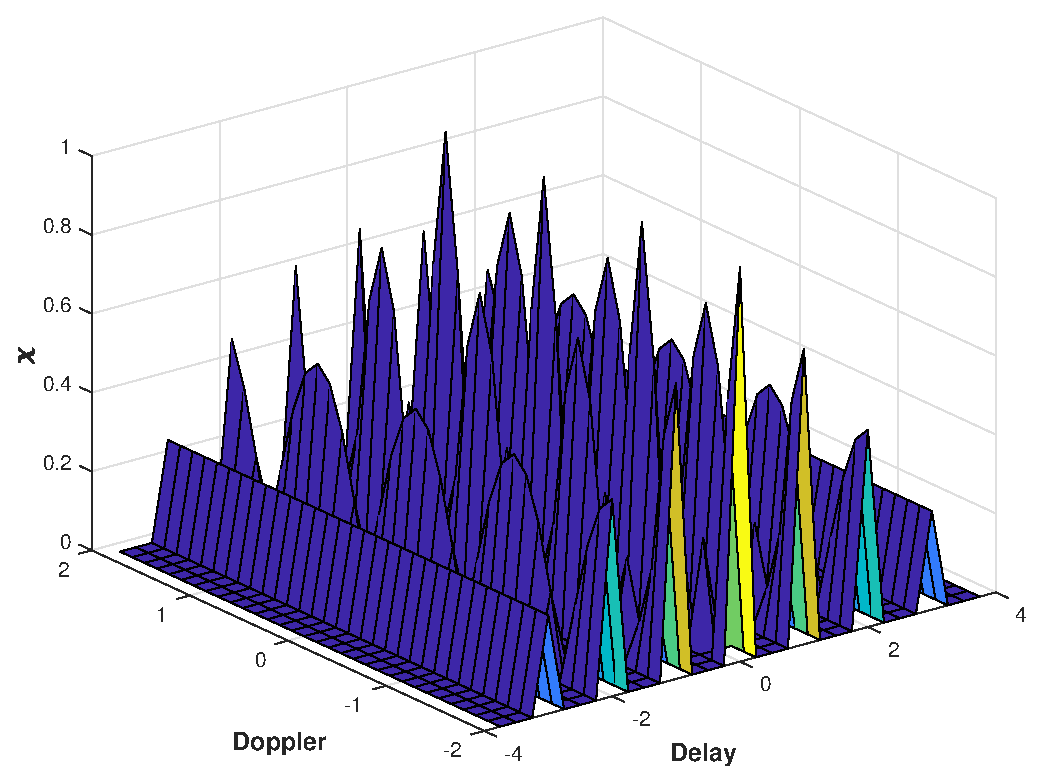
\includegraphics [width=4in]{LFM__01.eps}


\subsection*{(Zero delay response: Doppler cut)}

\begin{verbatim}
lfmwaveform = phased.LinearFMWaveform('SampleRate',4,'SweepBandwidth',1,'PRF',1,'PulseWidth', 0.25);


release(lfmwaveform);

lfmwaveform.NumPulses = 4;

wav = lfmwaveform();

figure(1);
ambgfun(wav,lfmwaveform.SampleRate,lfmwaveform.PRF, 'Cut', 'Delay');
title('Zero delay response (Doppler Cut)', 'FontSize', 12, 'FontWeight', 'bold')

figure(2);
ambgfun(wav,lfmwaveform.SampleRate,lfmwaveform.PRF, 'Cut', 'Doppler');
title('Zero doppler response (Range Cut)', 'FontSize', 12, 'FontWeight', 'bold');
\end{verbatim}

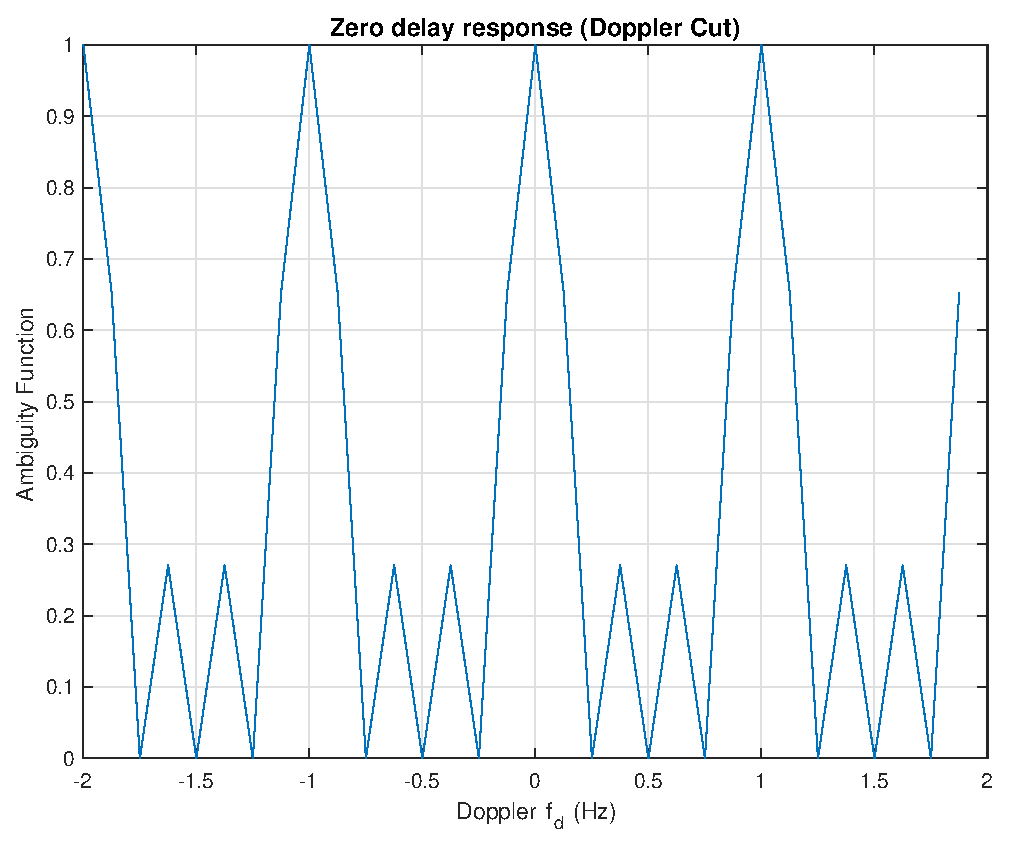
\includegraphics [width=4in]{LFM__02.eps}

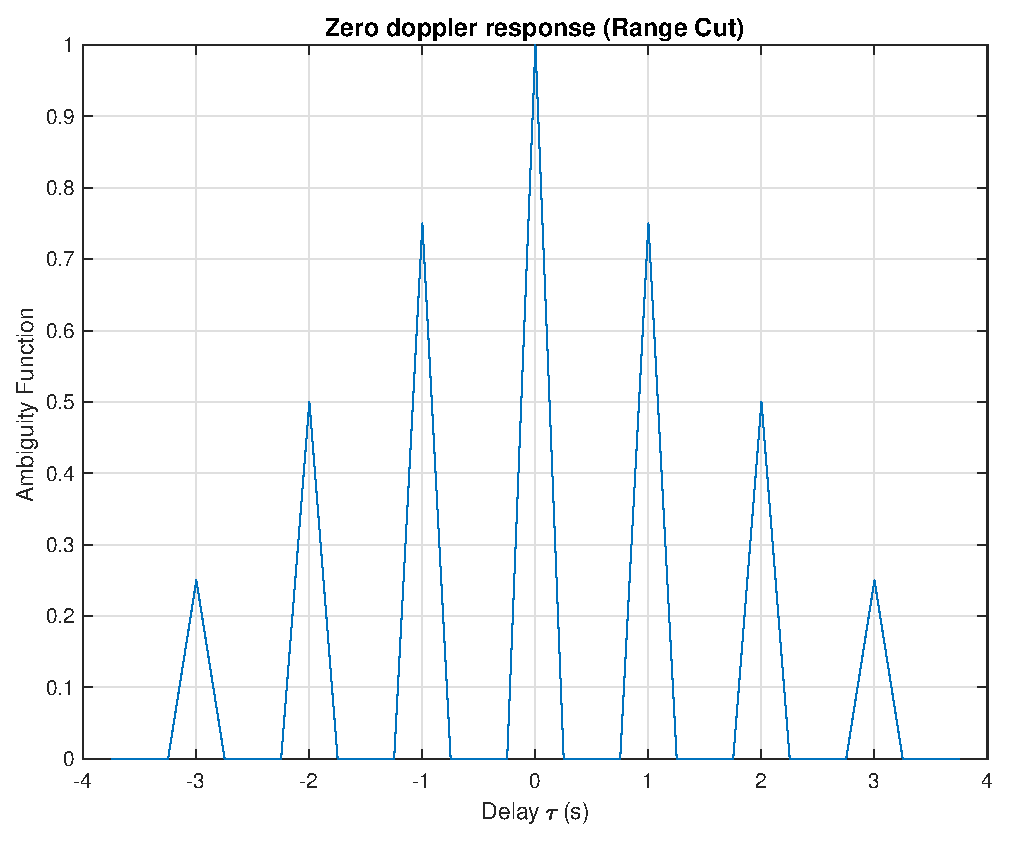
\includegraphics [width=4in]{LFM__03.eps}



\end{document}
    
